% Charles McEachern

% Fall 2015

% This is a template for writing a note to Bob in TeX. 

\documentclass{article}

% =============================================================================
% ==================================== Package List Copied from Thesis Template
% =============================================================================

\usepackage{epsfig} % Allows the inclusion of eps files
\usepackage{epic} % Enhanced picture mode
\usepackage{eepic} % Extensions for epic
\usepackage{units} % SI unit typesetting
\usepackage{url} % URL handling
\usepackage{longtable} % Tables that continue onto multiple pages
\usepackage{mathrsfs} % Support for \mathscr script
\usepackage{multirow} % Span rows in tables
\usepackage{bigstrut} % Space struts in tables up and down
\usepackage{amssymb} % AMS math symbols and helpers
\usepackage{graphicx} % Enhanced graphics support
\usepackage{setspace} % Adjust spacing in captions, single by default
\usepackage{xspace} % Automatically adjusting space after macros
\usepackage{amsmath} % \text, and other math formatting options
\usepackage{siunitx} % \num{} formatting and SI unit formatting
\usepackage{booktabs} % Enhanced tables with \toprule, etc.
\usepackage{hyperref} % Add clickable links to other parts of the document
\usepackage[noabbrev]{cleveref} % Automatically determine \cref type

\usepackage{parskip} % http://ctan.org/pkg/parskip

% Configure the siunitx package
\sisetup{
    group-separator = {,}, % Use , to separate groups of digits, like 12,345
    list-final-separator = {, and } % Always use the serial comma in \SIlist
}

% Configure the cleveref package
\newcommand{\creflastconjunction}{, and } % Always use the serial comma

\linespread{1.3}

% =============================================================================
% ================================================================= Definitions
% =============================================================================




% Names with special characters. 
\newcommand{\Alfven}{Alfv\'en\xspace}
\newcommand{\Ampere}{Amp\`ere\xspace}

% To make sure the capitalization is consistent. 
\newcommand{\ohmlaw}{Ohm's Law\xspace}
\newcommand{\amplaw}{\Ampere's Law\xspace}
\newcommand{\farlaw}{Faraday's Law\xspace}

% Field-aligned unit vectors. 
\newcommand{\xhat}{\ensuremath{\hat{x}}\xspace}
\newcommand{\yhat}{\ensuremath{\hat{y}}\xspace}
\newcommand{\zhat}{\ensuremath{\hat{z}}\xspace}

% Spherical unit vectors. 
\newcommand{\rhat}{\ensuremath{\hat{r}}\xspace}
\newcommand{\qhat}{\ensuremath{\hat{\theta}}\xspace}
\newcommand{\fhat}{\ensuremath{\hat{\phi}}\xspace}

% Use underlines for vectors and tensors. 
\renewcommand{\vec}[1]{\underline{#1}}
\newcommand{\tensor}[1]{\underline{\underline{#1}}}

% Differential operators. 
\newcommand{\dd}[1]{\ensuremath{ \frac{\partial}{\partial #1} }\xspace}
\newcommand{\ddt}{\dd{t}\xspace}
\newcommand{\curl}[1]{\ensuremath{ \nabla \times \vec{#1} }\xspace}
\renewcommand{\div}[1]{\ensuremath{ \nabla \cdot \vec{#1} }\xspace}
\newcommand{\grad}[1]{\ensuremath{ \nabla #1 }\xspace}

% Properly-scaled parentheses for grouping terms or for arguments. 
\newcommand{\lr}[1]{ \left( #1 \right) }
\newcommand{\lrsmall}[1]{ \left( {\scriptstyle #1} \right) }
\renewcommand{\arg}[1]{\!\lr{#1}}
\newcommand{\argsmall}[1]{\!\lrsmall{#1}}
\newcommand{\lrb}[1]{ \left[ #1 \right] }

% Circled plus-minus symbol. Solving quartics requires \pm and \opm. 
\newcommand{\opm}{ \text{ \textcircled{ \ensuremath{\hskip -0.2em \pm} } } \xspace}

% Define a better looking eV by moving the V slightly left
\DeclareSIUnit\electronvolt{e\hspace{-0.08em}V}

\DeclareSIUnit\RE{R_E}


\newcommand{\dt}{\ensuremath{\delta \hspace{-0.1em} t} \xspace}



% Azimuthal modenumber, typically indicated with a lowercase m. 
\newcommand{\azm}{\ensuremath{m_{azimuthal}}\xspace}

% Azimuthal modenumber, typically indicated with a lowercase m. 
\newcommand{\me}{\ensuremath{m_{e}}\xspace}

% Jacobian dererminant, typically indicated with a capital J, which we are using for current. 
\newcommand{\jac}{\ensuremath{D}\xspace}

% Dispersion tensor, typically indicated with... a capital D?
\newcommand{\dispersiontensor}{\tensor{T}\xspace}


% These things just get used a lot in the dispersion relation chapter...

% Boris-corrected speed of light. 
\newcommand{\cb}{\ensuremath{c_B} \xspace}

% Boris-corrected plasma frequency. 
\newcommand{\ob}{\ensuremath{\omega_B} \xspace}

% Boris-corrected electric constant. 
\newcommand{\eb}{\ensuremath{\epsilon_B} \xspace}

% Alfven speed. 
\newcommand{\va}{\ensuremath{v_A} \xspace}

% Perpendicular electric constant. 
\newcommand{\ep}{\ensuremath{\epsilon_\bot} \xspace}

% Epsilon zero. 
\newcommand{\ez}{\ensuremath{\epsilon_0} \xspace}

% Conductivities. 
\newcommand{\sz}{\ensuremath{\sigma_0} \xspace}
\newcommand{\sh}{\ensuremath{\sigma_H} \xspace}
\renewcommand{\sp}{\ensuremath{\sigma_P} \xspace}




\newcommand{\spe}{\ensuremath{\frac{\sigma_P}{\ep}} \xspace}
\newcommand{\she}{\ensuremath{\frac{\sigma_H}{\ep}} \xspace}




% 3x3 matrix. 
\newcommand{\mmm}[9]{ \left[ \begin{array}{ccc}
    #1 & #2 & #3 \\
    #4 & #5 & #6 \\
    #7 & #8 & #9
  \end{array} \right] }

% 2x2 matrix. 
\newcommand{\mm}[4]{ \left[ \begin{array}{cc}
    #1 & #2 \\
    #3 & #4
  \end{array} \right] }

% 2x1 matrix, or 2-vector. 
\newcommand{\vv}[2]{ \left[ \begin{array}{c}
    #1 \\
    #2
  \end{array} \right] }


% Physics constants
\newcommand{\C}{{\mathrm{c}}}

% Add space between rows of tables
\newcommand{\spacerows}[1]{\renewcommand{\arraystretch}{#1}}









% =============================================================================
% ======================================================== Document Starts Here
% =============================================================================

\begin{document}

% -----------------------------------------------------------------------------
% -----------------------------------------------------------------------------
% -----------------------------------------------------------------------------
\section{Model Summary}

We start with \farlaw, \amplaw, and \ohmlaw. Driving is delivered through an additional current term in \amplaw (usually sinusoidal). We consider electron inertial effects in the parallel component of \ohmlaw. 
\begin{align*}
  \ddt \vec{B} & = - \curl{E}
  &
  \tensor{\epsilon} \cdot \ddt \vec{E} & = 
    \frac{1}{\mu_0} \lr{ \curl{B} } - \vec{J}_{drive} - \vec{J}
  \\
  \vec{J}_\bot & = \tensor{\sigma}_\bot \cdot \vec{E}_\bot
  &
  \ddt J_\parallel & = \frac{n e^2}{\me} E_\parallel - \nu J_\parallel
\end{align*}

We use a two-dimensional dipole grid spanning $2 \lesssim L \lesssim 10$. Field lines end at a fixed altitude, taken to be the ionospheric current sheet, at an altitude of $\sim \SI{100}{\km}$. Grid spacing is fine at the ionosphere and coarse at large distances. 
%\begin{figure}[h!]
%  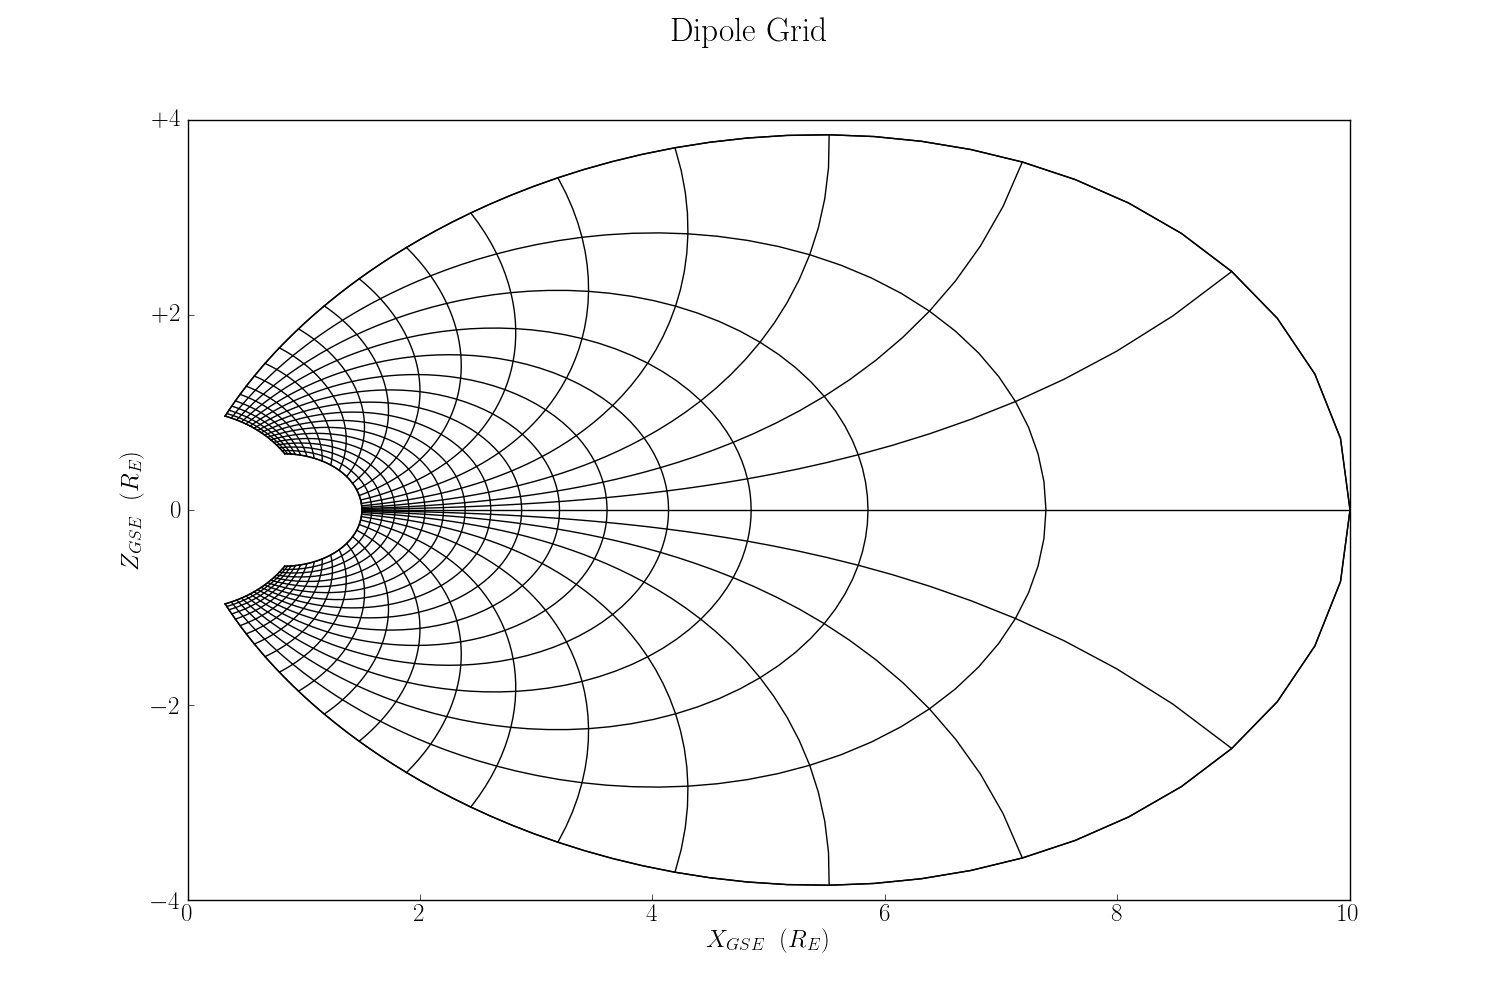
\includegraphics[width=5in]{grid.png}
%  \caption{Illustration of the relative spacing of grid points along the dipole. }
%  \label{grid}
%\end{figure}

At the boundary, we assume an insulating atmosphere and a conducting Earth. This allows us to compute a scalar magnetic potential, $\Psi$, and from it $B_\phi$ and $B_\theta$ at $R_E$ and $R_I$. We use the jump in horizontal magnetic field over the ionospheric current sheet as a boundary condition on the horizontal electric field. %. Each time step, we use $B_r$ to compute $\Psi$ in terms of spherical harmonics. We then use $\Psi$ to compute $B_\phi$ and $B_\theta$ at $R_E$ and $R_I$. From the jump in magnetic field over the ionospheric current sheet, we compute boundary values for the horizontal electric field. 
\begin{align*}
  \mu_0 \tensor{\Sigma} \cdot \vec{E} & = \hat{r} \times \Delta \! \vec{B} 
\end{align*}

The simulation runs in two and a half dimensions, resolving a meridional slice of the magnetosphere. Perpendicular derivatives assume that all fields vary azimuthally per $\exp \arg{i m \phi}$. This should not be read as a periodic oscillation which continues all the way around the Earth. Rather, we selectively consider phenomena which are localized in MLT, and let $m$ dictate their azimuthal wavelength. The real component of a field is taken to be its value at our meridional slice, while the imaginary component is azimuthally phase shifted. %In practice, driving with azimuthal ``current'' (delivered to the azimuthal electric field) produces real poloidal field components ($B_x$ and $E_y$) and imaginary toroidal field components ($B_y$ and $E_x$). 

We use static profiles for conductivity, \Alfven speed, number density, and so on. Different profiles are used to simulate the dayside or nightside during quiet or active times. 

% -----------------------------------------------------------------------------
% -----------------------------------------------------------------------------
% -----------------------------------------------------------------------------
\section{Model Uses}

Past work with this model (or ones very much like it) have used compressional driving -- an enhancement of $B_z$ along the outer boundary -- to simulate ULF waves. Recent work (Jesse's 2010 thesis, Bob's 2013 paper) has focused in particular on IAR modes, frequencies $\sim \SI{1}{\s}$. 

My work instead focuses on Pc4 pulsations -- field line resonances just outside the plasmasphere. Pc4s can exhibit large azimuthal modenumbers, which makes them hard to resolve in a fully 3D simulation. Additionally, high-$m$ \Alfven waves cannot be driven compressionally in this frequency range. As the azimuthal wavelength shrinks, the azimuthal wavenumber grows, and so does the minimum non-evanescent \Alfven wave frequency. 

Ideally, the results from this model can be compared to the recent work by RBSP: ``Storm time occurrence and spatial distribution of Pc4 poloidal ULF waves in the inner magnetosphere: A Van Allen Probes statistical study'' by Dai et al, 2015. 

% -----------------------------------------------------------------------------
% -----------------------------------------------------------------------------
% -----------------------------------------------------------------------------
\section{Model Output}

The model simulates electric fields, magnetic fields, and currents along the dipole grid, broken up into parallel, perpendicular, and azimuthal components. Horizontal magnetic fields are also computed at the top and bottom of the atmosphere. This data can be visualized in a handful of ways. 

% -----------------------------------------------------------------------------
% -----------------------------------------------------------------------------
% -----------------------------------------------------------------------------
\section{Snapshots in Time}

We can produce snapshots in time of field evolution over the entire dipole. 

These can also be animated (in principle). 

% -----------------------------------------------------------------------------
% -----------------------------------------------------------------------------
% -----------------------------------------------------------------------------
\section{Ground Signatures}

Contour plot. 

Line plot at a single location. 





\begin{figure}[h!]
  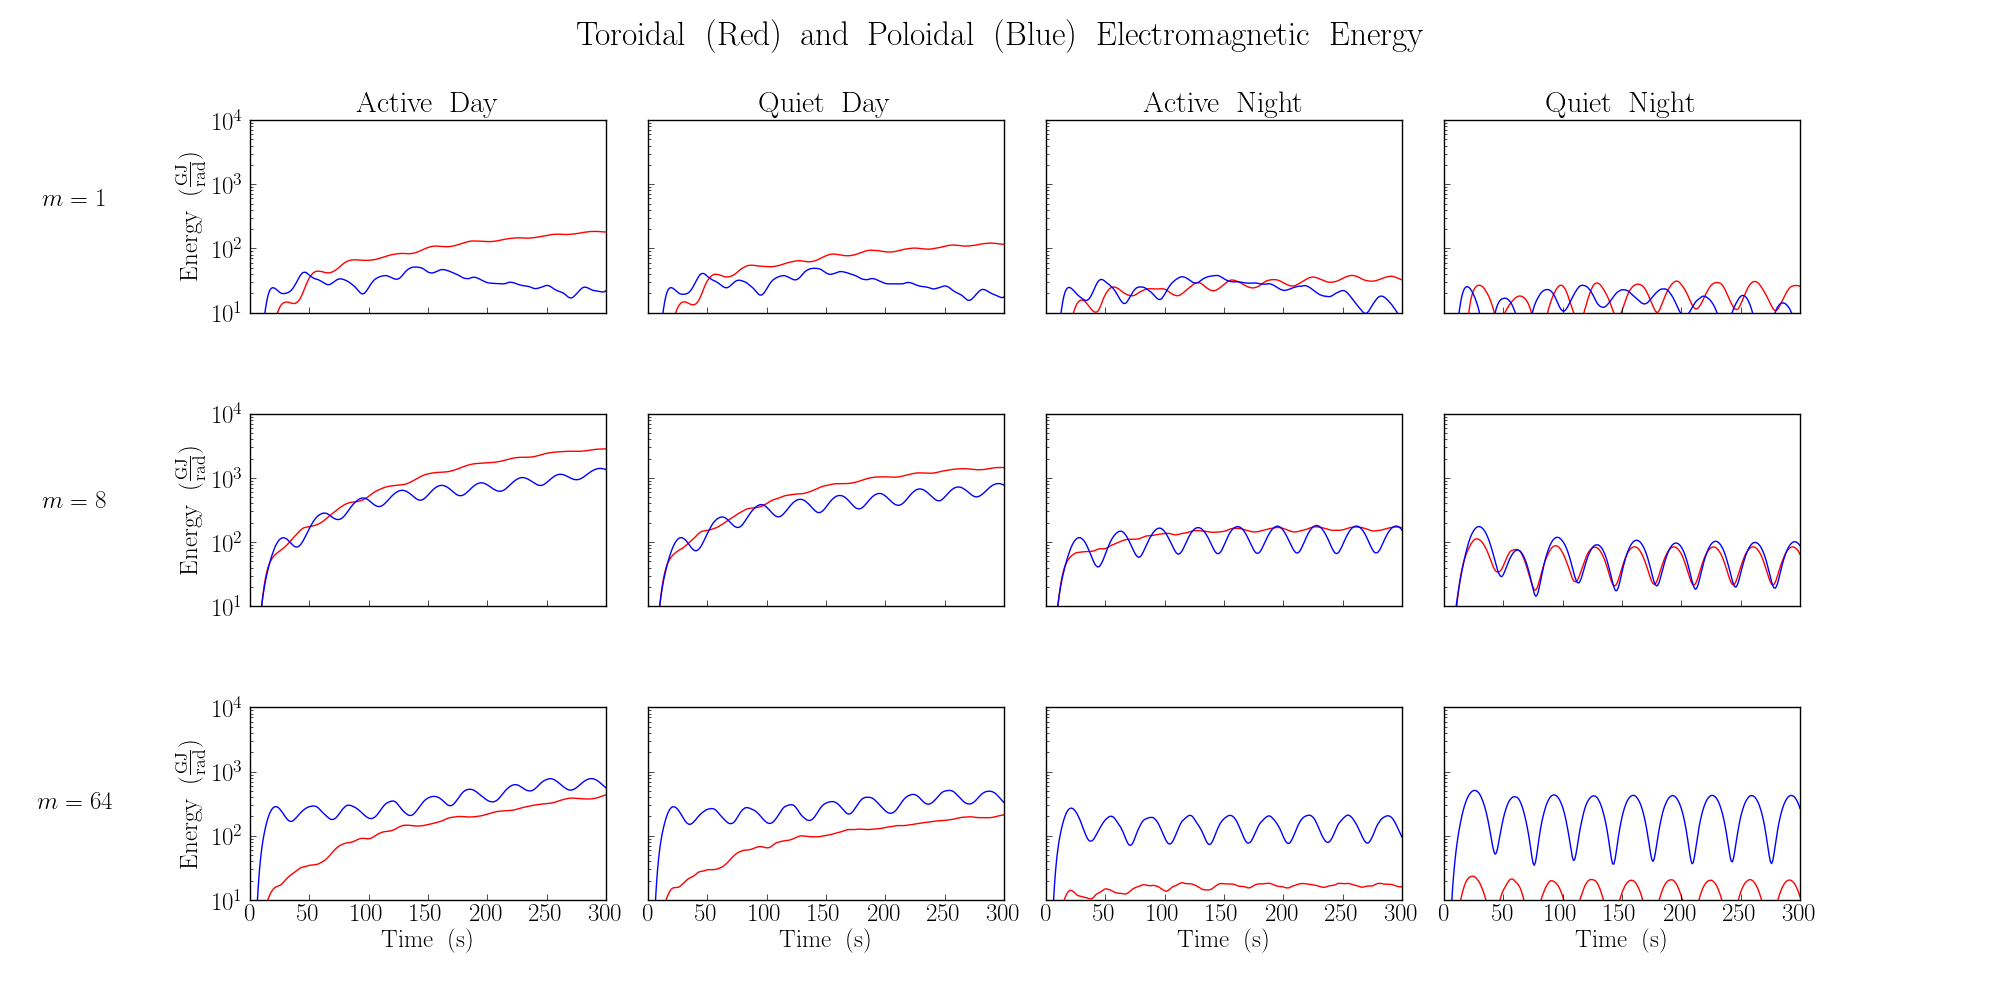
\includegraphics[width=5in]{energy.png}
  \caption{Poloidal-toroidal coupling depends on both modenumber and conductivity. }
\end{figure}





% -----------------------------------------------------------------------------
% -----------------------------------------------------------------------------
% -----------------------------------------------------------------------------
\section{``In Situ'' Plots}




We can follow the time evolution of field components at a small number of specific locations. 




\begin{figure}[h!]
  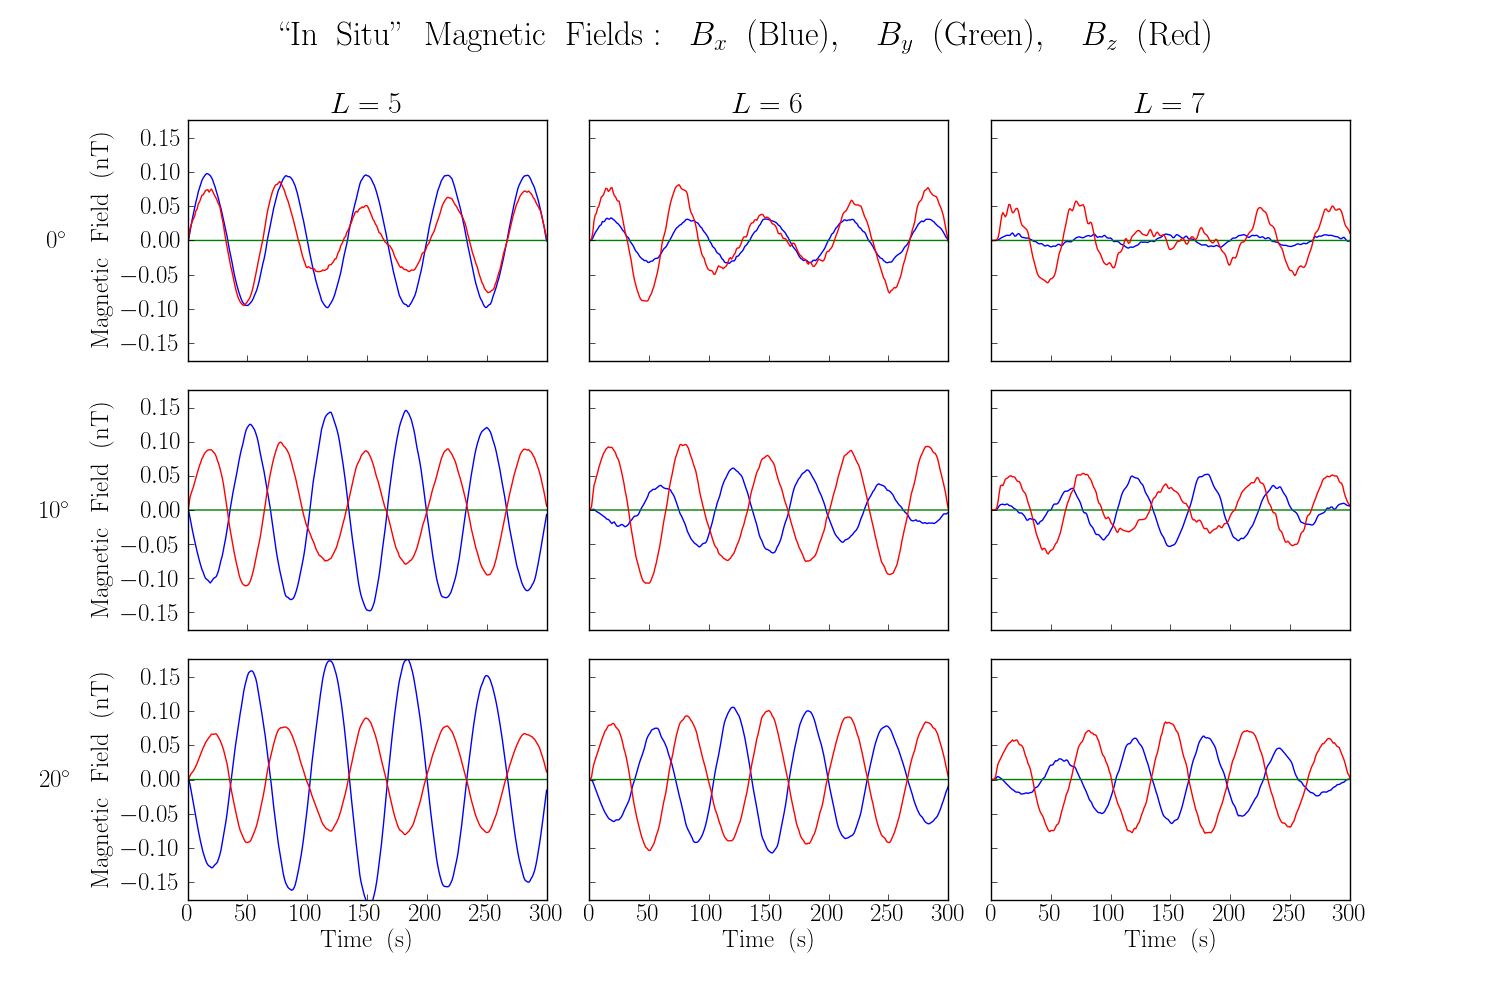
\includegraphics[width=5in]{insitu.png}
  \caption{Magnetic fields over time for a stationary observer. }
\end{figure}




\begin{figure}[h!]
  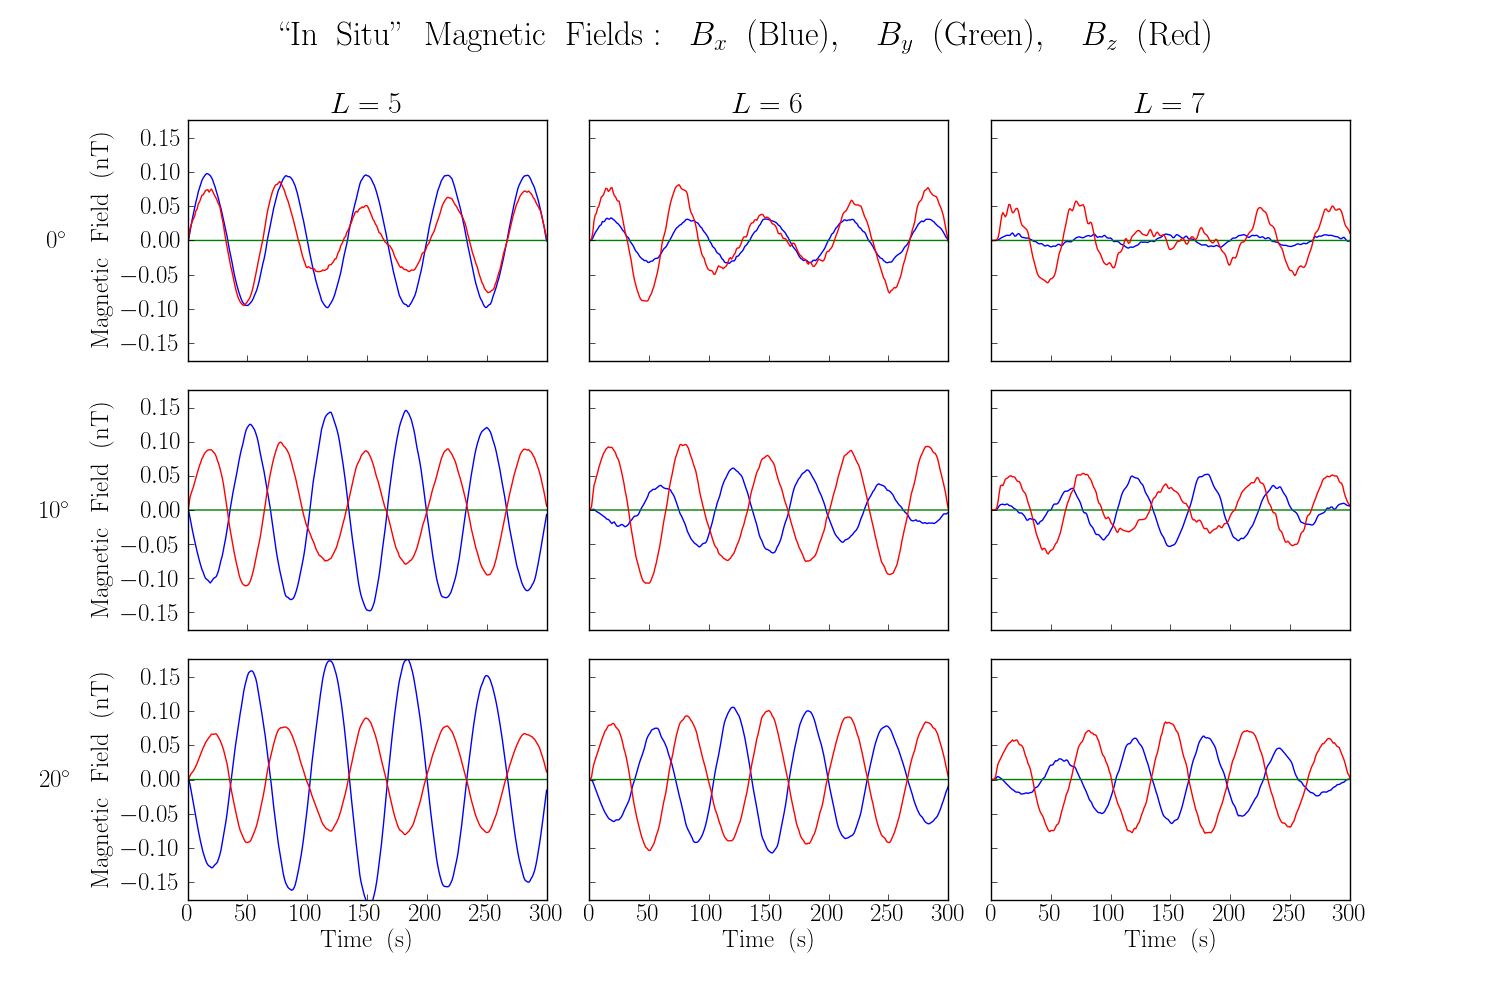
\includegraphics[width=5in]{insitu.png}
  \caption{Magnetic fields over time for an observer moving at \SI{1}{\km/\s}. }
\end{figure}



Speed is a significant consideration with this model. Because many runs can be performed in a relatively short amount of time, we generally conduct an ensemble of similar runs rather than a single parge run. This helps us distinguish broad trends from individual oddities. 









%The parallel electric field, and all components of the magnetic field, are updated directly. Perpendicular currents are eliminated. Perpendicular electric fields and the parallel current are solved with integrating factors. 
%\begin{align*}
%  \vec{E}_\bot \! \arg{\dt} & = 
%    \tensor{R} \argsmall{\frac{\sigma_H}{\epsilon_\bot} \dt} \cdot \vec{E}_\bot \! \arg{0}
%      \exp \argsmall{-\frac{\sigma_P}{\epsilon_\bot} \dt}
%    + \dt \tensor{R} \argsmall{\frac{\sigma_H}{\epsilon_\bot} \frac{\dt}{2} } \cdot  \vec{F}_\bot \! \argsmall{ \frac{\dt}{2} } \exp \argsmall{-\frac{\sigma_P}{\epsilon_\bot} \frac{\dt}{2} }
%  \\
%  J_\parallel \arg{\dt} & = 
%    J_\parallel \arg{0} \exp \arg{ -\nu \dt }
%    + \frac{n e^2}{\me} \dt \, E_\parallel \argsmall{\frac{\dt}{2}}  
%    \exp \argsmall{ -\nu \frac{\dt}{2} }
%\end{align*}

%where
%\begin{align*}
%  \vec{F} \equiv \frac{1}{\mu_0 \epsilon_\bot} \curl{B} - \frac{1}{\epsilon_\bot} \vec{J}_{drive}
%  \qquad \text{and} \qquad
%  \tensor{R} \arg{\theta} \equiv \mm{\cos\theta}{-\sin\theta}{\sin\theta}{\cos\theta}
%\end{align*}



\end{document}













